\section{Methodology}
\label{sec:methodology}

\comments{
In this section, we introduce key steps of our works. We first detail how the architecture of SketchPointNet is designed. Next, we will show how to resample each sketch into a fixed number of points. At last, we explain that our group scheme guarantees the integrity of group patterns.}

In this section, we will first introduce the network architecture of our SketchPointNet. Next, we describe the algorithm details of point sampling and grouping from sketch strokes, and the network to extract both local and global patterns for recognition.


%\subsection{Architecture of SketchPointNet}
%\label{ssec:sketch_point_net}

\para{Architecture of SketchPointNet.}
Fig.~\ref{fig:sketchpointnet} shows the architecture of our SketchPointNet.
%SketchPointNet recognizes sketches as time series. \cxj{Do you input the points as sequence?}
%
The directly captured stroke paths from various input devices are typically contact points that distribute unevenly along strokes with different movement speeds and device sizes.
To make them directly comparable, we resample the input sketch $\mathcal{S}$ into $N$ evenly distributed points as a point set $\mathbb{P}=\{P_i|i=1,\ldots,N\}$.
%Moreover, the current Tensorflow only supports static graphs. Resampling the input sketch into a fixed number of points makes the implementation simple.
A transformation net is employed to estimate a $3\times3$ affine transformation matrix to align the input sketch, similar with PointNet~\cite{qi2017pointnetplusplus}.
%
Given the resampled and rectified point set, we extract the sketch features hierarchically with three networks~(PN-1, PN-2, PN-3) from low level to global level.
%
In each level, we group the sampled point set $\ptset$ into $K_g$ groups according to their spatial and temporal neighborhood in different size.
Stroke patterns are extracted using a mini PointNet~\cite{qi2017pointnetplusplus} for each point group.
%
From the global pattern extracted by the third PointNet (PN-3), a multilayer perceptron is then employed to predict the scores for the $N_{class}$ sketch categories.



While the overall architecture of our SketchPointNet is similar with PointNet++~\cite{qi2017pointnetplusplus}, the main difference lies on the sampling and grouping procedure.
Targeting at 3D point clouds, PointNet++~\cite{qi2017pointnetplusplus} considers the spatial distribution of points in the 3D space.
In contrast, not only the spatial pattern is important, the temporal pattern is also important for sketch recognition.
%
During our sampling and grouping, the temporal and spatial information is integrated together to extract sketch patterns for robust recognition.
\\


%\subsection{Point Sampling}
%\label{ssec:resample}
\para{Point sampling.}
%% key concept of resampling is to preserve local temporal and spatial relations
To make various sketches comparable, we sample $N_{pt}$ equidistantly spaced points along strokes.
By sampling along strokes, the temporal information is encoded in the point distribution.
%
The length of each stroke is calculated and the total length of all strokes is $L_{sum}=\sum^{M}_{i=1} L_i$, where $M$ is the stroke number.
%
Given the desired point number $N_{pt}$, we assign each stroke $N_i=\frac{L_i}{L_{sum}}N_{pt}$ points according to its stroke length $L_i$.
Then we reample each stroke into $B_i$ points equidistantly along the stroke.
%
Fig.~\ref{fig:resample} shows the sampling results with different number of points.
We can see that the main structure is well preserved during the sampling procedure without losing much details, even with a very small number (N=128) of points.
\\

\begin{figure}
	\center
	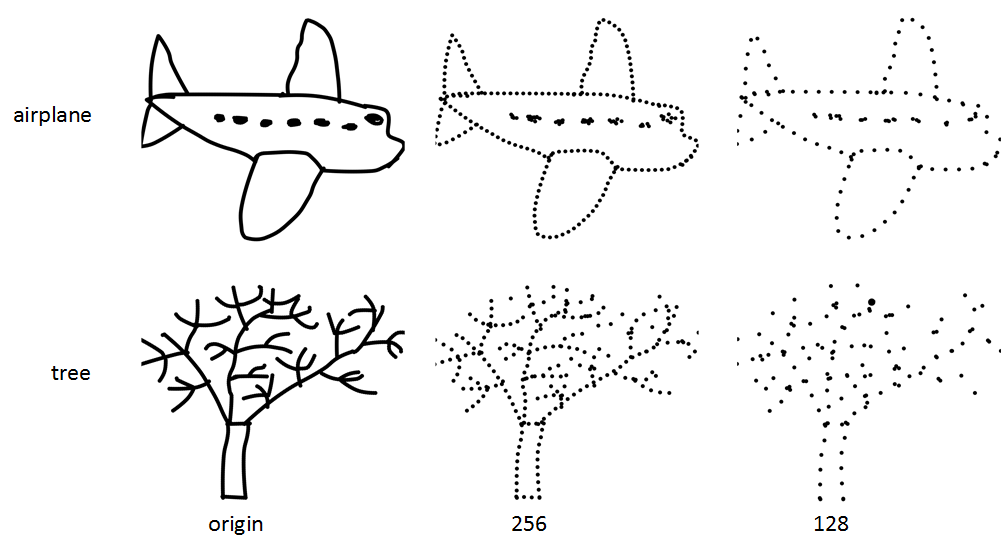
\includegraphics[width=3in]{images/resample2.png}
	\fcaption{Sketch resampling with different number of points. Each continuous stroke is shown in a unique color.}
	\label{fig:resample}
\end{figure}



%\subsection{Point Grouping}
%\label{ssec:group_scheme}

\para{Point grouping.}
To extract features of the input sketch, we group a set of points on the strokes and feed them into a PointNet, which is flexible for the number of input points.
%
Given a desired number of groups $N_{group}$ at a certain level, we first sample $N_{group}$ points as the group centers from the input sketch using the sampling method described above.
%
Then for each group, we extract a set of points equidistantly on the input strokes in an area of radius $r$ surrounding the group center.
%
The number $K_{group}$ of points in different groups varies over the sketch region. We set an upper bound for $K_{group}$ to reduce the computational complexity.
%While the sketch is first re-sampled evenly distributed temporarily in the previous sampling step, the point density is not even in the spatial domain.
%We sample the partial sketch in a local region to a number $K_{group}$ of points equidistantly.
%
As Fig.~\ref{fig:group} shows, the points in a local region with different radius present different local patterns.
%
Both temporal and spatial patterns are preserved during the grouping procedure, which are essential for sketch recognition.
\\



\begin{figure}
	\centering
	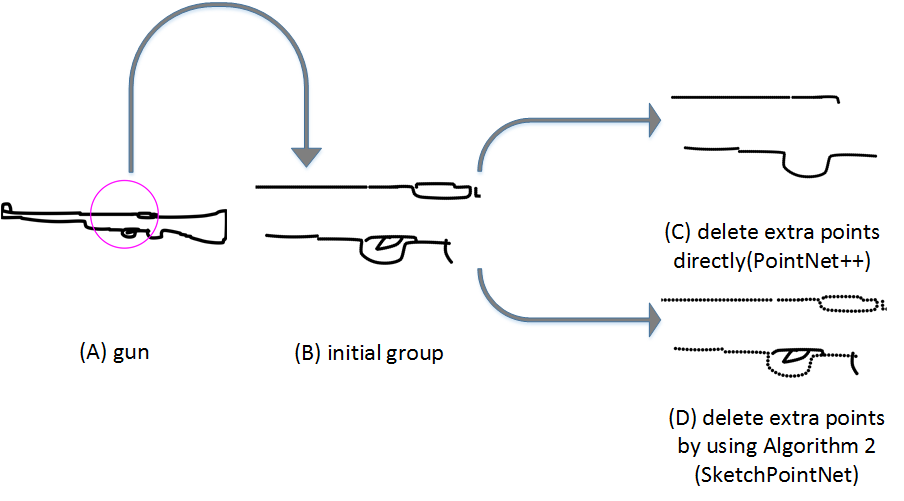
\includegraphics[width=\columnwidth]{images/group.png}
	\fcaption{Comparison of dealing with extra points.}
	\label{fig:group}
\end{figure}

\begin{figure}
	\centering
	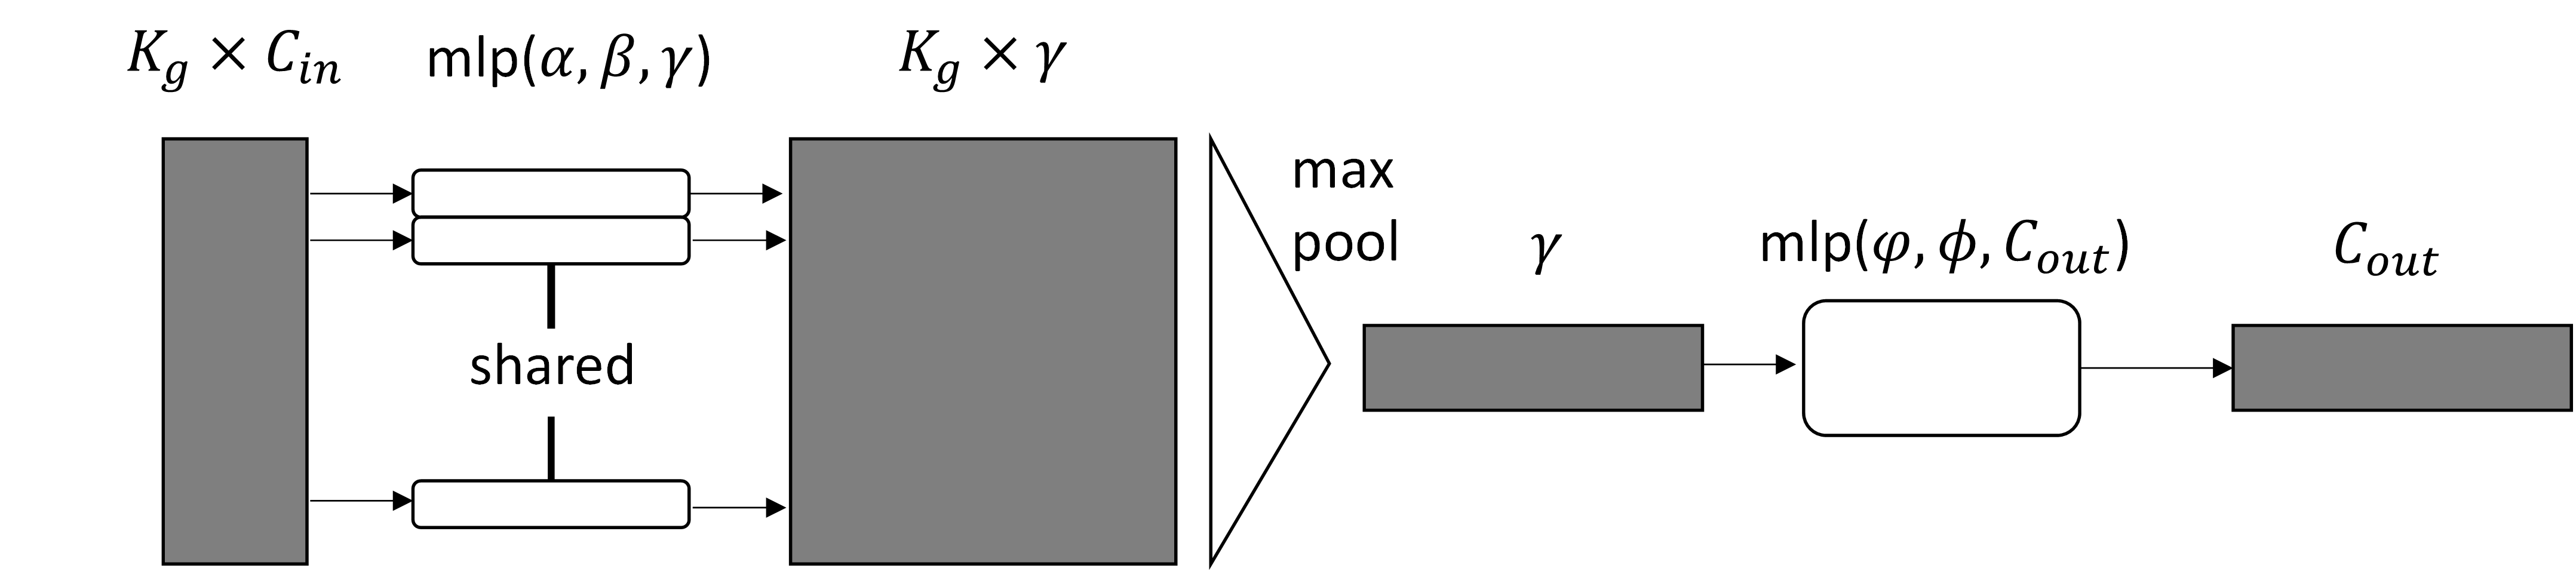
\includegraphics[width=\columnwidth]{images/pointnet.png}
	\caption{Architecture of our mini PointNet.}
	\label{fig:miniPN}
\end{figure}
%\subsection{Group Pattern Extraction}
\para{Pattern extraction.}
%
We use a modified version of the PointNet~\cite{qi2017pointnet} to extract the sketch pattern in a local region that contains a flexible number of points.
The architecture of our mini PointNet is shown in Fig.~\ref{fig:miniPN}.
%
%After the point grouping step, we feed a mini PointNet with $N_g$ groups with data size $N_g \times K_g \times C$ to extract the sketch pattern for recognition.
%
For each group, a mini PointNet is fed with $K_g$ points in its local region with data size $K_g \times C_{in}$.
Here, $K_g$ is the number of points in a group, and $C$ is the number of data channel of each point.
Each mini PointNet consists three parts.
The first part is $K_g$ shared-weight three-layer perceptrons (with $M^{1}_1$,$M^{1}_2$,$M^{1}_3$ neurons at each layer respectively), which converts the input data of each points into another feature space.
%
The second part is a max-pooling layer to aggregate features of the $K_g$ points into a fixed-dimension feature.
%
The third part is a three-layer perceptron (with $M^{2}_1$,$M^{2}_2$,$M^{2}_3$ neurons at each layer respectively).
%
The output of the mini PointNet is a $C_{out}=M^{2}_3$ dimensional feature vector.
%Here, $N_g$ is the number of local groups, $K_g$ is the number of points in each group, $C$ is the number of data channel of each point.


Initially, we have the 2{D} coordinates and stroke order of each point for the normalized sketch.
We translate each point into a local frame relative to the center point of each group.
Therefore, the data channel $C^1_{in}=2+1$ for the first PointNet PN-1, including the 2D local coordinates and 1-D stroke order.
The output of PN-1 is a $C^1_{out}$ dimensional feature vector for each group.
%
Different with PointNet++~\cite{qi2017pointnetplusplus} for 3D point clouds, the stroke order does matters for sketch recognition, because human typically draw the overall shape and then add fine details later.
%
The strokes drawn earlier have more impact effects for recognizing a coarse sketch.
%

Then, increasing the radius $r_2$ for grouping points, which is equivalent to increasing the receptive field, we extract sketch patterns in a higher level.
%
Therefore, for the second PointNet PN-2, the input is the $K_{g2} \times C^2_{in}$ data, where $K_{g2}$ is the number of points in the local region of a group, $C^2_{in}=2+1+C^1_{out}$ for each group, including the 2-D local coordinate of the group center, 1-D stroke order and the $C^1_{out}$-D feature extracted for the local region from the first PointNet.
%
The output of PN-2 is a $C^2_{out}$-D feature vector for each group.
\\

\para{Sketch classification.}
%\label{ssec:classification}
After the two-level local pattern extraction, we feed the $N_{g2} \times C^2_{out}$ data into the third mini PointNet PN-3, which produces $C^{3}_{out}=N_{class}$ dimensional vector as the predicted scores for the $N_{class}$ categories.




